\documentclass[tikz]{standalone}
\usetikzlibrary{positioning}
\usetikzlibrary{decorations.pathmorphing} % noisy shapes
\usetikzlibrary{fit}                                   % fitting shapes to coordinates
\usetikzlibrary{backgrounds}   % drawing the background after the foreground

\tikzstyle{background}=[rectangle,
                                                fill=blue!10,
                                                inner sep=0.2cm,
                                                rounded corners=5mm]
\tikzstyle{matrx}=[rectangle,
                                    thick,
                                    minimum size=1cm,
                                    draw=gray!80,
                                    fill=gray!20]

\tikzstyle{arrow} = [thick,->,>=stealth]


\begin{document}
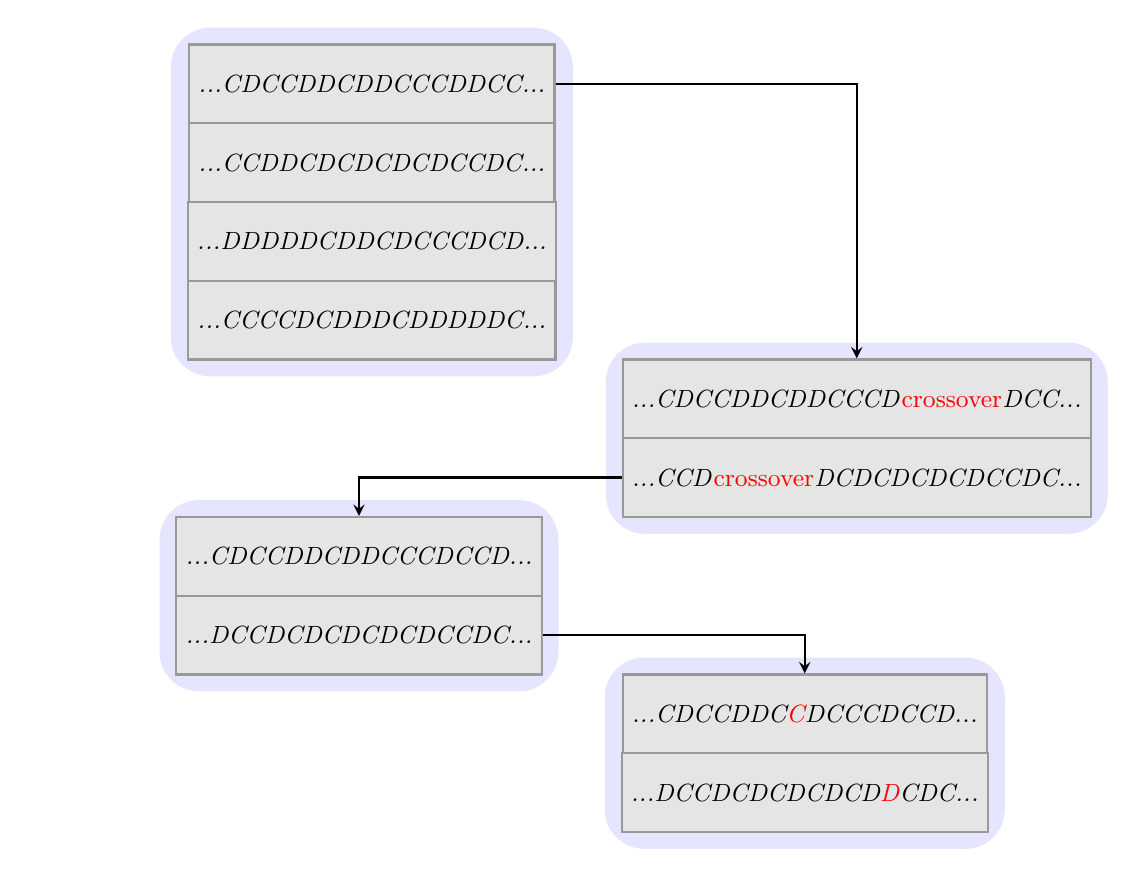
\begin{tikzpicture}[scale=2]

  \node (table1) [matrx]{\small\textit{...CDCCDDCDDCCCDDCC...}};
  \node (table2) [matrx, below of=table1]{\small\textit{...CCDDCDCDCDCDCCDC...}};
  \node (table3) [matrx, below of=table2]{\small\textit{...DDDDDCDDCDCCCDCD...}};
  \node (table4) [matrx, below of=table3]{\small\textit{...CCCCDCDDDCDDDDDC...}};
  % Second line: System noise & input matrix
  \node (cross1) [matrx, right=of table4, yshift=-1cm, xshift=-5]{\small\textit{...CDCCDDCDDCCCD}\textcolor{red}{crossover}\small\textit{DCC...}};
  \node (cross2) [matrx, below of=cross1] {\small\textit{...CCD}\textcolor{red}{crossover}\small\textit{DCDCDCDCDCCDC...}};

  %children
  \node (child1) [matrx, left=of cross2, yshift=-1cm]{\small\textit{...CDCCDDCDDCCCDCCD...}};
  \node (child2) [matrx, below of=child1] {\small\textit{...DCCDCDCDCDCDCCDC...}};
  %mutation
  \node (mutan1) [matrx, right=of child2, yshift=-1cm]{\small\textit{...CDCCDDC\textcolor{red}{C}DCCCDCCD...}};
  \node (mutan2) [matrx, below of=mutan1] {\small\textit{...DCCDCDCDCDCD\textcolor{red}{D}CDC...}};

  \begin{pgfonlayer}{background}
    \node [background,
                fit=(table1) (table2) (table3) (table4),
                label=left:\textcolor{white}{Parents:}] {};
    \node [background,
                fit=(cross1) (cross2),
                label=left:\textcolor{white}{Crossovers:}] {};
    \node [background,
                fit=(child1) (child2),
                label=left:\textcolor{white}{Children:}] {};
    \node [background,
                fit=(mutan1) (mutan2),
                label=left:\textcolor{white}{Mutation:}] {};
  \end{pgfonlayer}

  \draw [arrow] (table1) -| (cross1);
  \draw [arrow] (cross2) -| (child1);
  \draw [arrow] (child2) -| (mutan1);
\end{tikzpicture}
\end{document}